%%% DOCUMENT SETUP %%%
\documentclass[11pt,a4paper]{article}
\usepackage[english]{babel}

%%% LAYOUT %%%
\usepackage{fullpage}
\usepackage[parfill]{parskip}
\usepackage{multicol}
\usepackage{footnote}

%%% GRAPHICS %%%
\usepackage{graphicx}
\usepackage{color}
\usepackage{graphics}
\usepackage{rotating}
\usepackage{subfig}
\usepackage{amsmath}
\usepackage{amssymb}
\usepackage{amscd}
\usepackage{xfrac}
\usepackage{float}
\usepackage{dsfont}

%%% FONT %%%
\usepackage{ifxetex}
\ifxetex
  \usepackage{fontspec}
    \setmainfont{Linux Libertine O}
  \usepackage{xunicode}
  \usepackage{microtype}
\else
  \usepackage[T1]{fontenc}
  \usepackage[latin1]{inputenc}
  \usepackage{times}
  \usepackage{microtype}
\fi

%%% Coding %%%
\usepackage{listings}
\usepackage{pseudocode}

%%% TITLE PAGE %%%
\author{Jeroen Hofman \ \ \ \ \ Carlo Kuiper\\
[15pt] University of Amsterdam (\textsc{UvA})}

\title{Computational Finance\\
Assignment III: Finite-Difference Methods for Option Pricing}

\begin{document}
\maketitle
\captionsetup{width=0.8\textwidth}
\thispagestyle{empty}

%%% TABLE OF CONTENTS %%%
\newpage
\tableofcontents
\newpage

\section{Introduction}
In this last assignment we investigate finite-difference methods for option pricing, specifically we derive finite difference approximations for the Black-Scholes PDE and use these approximations to compute the option price for an European call. We compare different step sizes for the time and spatial coordinate of the PDE and look at stability and convergence of the solution. We also use the finite difference schemes to give approximations for $\delta$, the hedge parameter.

\section{Theory}

\subsection{Discretization of the BS-PDE}

We will derive two finite difference schemes for option pricing from the Black-Scholes equation: the Forward Time Centered Scheme (FTCS) and the Cranck Nicolson Scheme (CN).  The general idea is to estimate the partial differentials in the Black-Scholes equation. Since these are partial derivatives of the option price with respect to time and underlying, the estimation will converge to the true solution for decreasing time steps and decreasing underlying steps in certain ratios. The partial differentials can be solved forward or backward in time. They are estimated by truncating a Taylor expansion. Finite difference methods might seem inconvenient, however they are actually useful in pricing exotic options. Sometimes it is uncertain if trees or Monte Carlo simulations converge, then finite difference methods provide a good alternative.

The Black-Scholes Partial Differential Equation (BS-PDE) derived for a plain vanilla option has the following form

\begin{equation}
\frac{\partial V}{\partial t}+rS\frac{\partial V}{\partial S}+\frac{1}{2}\sigma^2S^2\frac{\partial^2V}{\partial S^2}=rV
\label{eq:BS-PDE}
\end{equation}

The equation can be transformed into a PDE with constant coefficients, by introducing $X=\ln S$. Since the equation is commonly solved backwards in time, it is for further numerical treatment convenient to introduce the following transformation

\begin{equation*}
\frac{\partial V}{\partial t}=-\frac{\partial V}{\partial \tau}
\end{equation*}

We obtain the other expressions for the transformed partial differentials with a little calculus

\begin{align*}
\frac{\partial V}{\partial S}&=\frac{\partial X}{\partial S}\frac{\partial V}{\partial X}=\frac{1}{S}\frac{\partial V}{\partial X}\\
\frac{\partial^2 V}{\partial S^2}&=\frac{\partial}{\partial S}\left(\frac{1}{S}\frac{\partial V}{\partial X}\right)=\frac{1}{S}\frac{\partial^2 V}{\partial X^2}-\frac{1}{S^2}\frac{\partial V}{\partial X}\\
\end{align*}

Substituting these expression into the BS-PDE yields the transformed BS-PDE:

\begin{equation}
\frac{\partial V}{\partial \tau}=\left(r-\frac{1}{2}\sigma^2\right)\frac{\partial V}{\partial X}+\frac{1}{2}\sigma^2\frac{\partial^2V}{\partial X^2}-rV
\label{eq:transformed-BS-PDE}
\end{equation}

The explicit FTCS for the transformed BS-PDE can be derived by means of Taylor Expansion Techniques. Recalling the following Taylor expansions 

\begin{align}
V(X+\Delta X,\tau)&=V(X,\tau)+\Delta X\frac{\partial V(X,\tau)}{\partial X}+\frac{1}{2!}\Delta X^2 \frac{\partial^2 V(X,\tau)}{\partial X^2}+\ldots \label{eq:TaylorminDeltaX}\\
V(X-\Delta X,\tau)&=V(X,\tau)-\Delta X\frac{\partial V(X,\tau)}{\partial X}+\frac{1}{2!}\Delta X^2 \frac{\partial^2 V(X,\tau)}{\partial X^2}-\ldots \label{eq:TaylorDeltaX} \\
V(X,\tau+\Delta \tau)&=V(X,\tau)+\Delta \tau \frac{\partial V(X,\tau)}{\partial X}+\frac{1}{2!}\Delta \tau^2 \frac{\partial^2 V(X,\tau)}{\partial X^2}+\ldots \label{eq:TaylorDeltaTau}
\end{align}

Subtracting (\ref{eq:TaylorminDeltaX}) from (\ref{eq:TaylorDeltaX}) we get a centered approximation for the partial derivative of $V$ to $X$ with a truncation error of order $\mathcal{O}(\Delta X^2)$

\begin{equation}
\frac{\partial V}{\partial X}\approx \frac{V(X+\Delta X,\tau)-V(X-\Delta X,\tau)}{2\Delta X}
\label{eq:centeredDeltaX}
\end{equation}

Combining (\ref{eq:TaylorDeltaX}) and (\ref{eq:TaylorminDeltaX}) yields a centered approximation for the second order partial derivative of $V$ to $X$ with a truncation error of order $\mathcal{O}(\Delta X^2)$

\begin{equation}
\frac{\partial^2 V}{\partial X^2}\approx \frac{V(X+\Delta X,\tau)-2V(X,\tau)+V(X+\Delta X,\tau)}{\Delta X^2}
\label{eq:centeredDeltaXkwadraat}
\end{equation}

Finally we obtain from (\ref{eq:TaylorDeltaTau}) a forward approximation (actually a backward approximation since $\Delta \tau$ goes back in time) for the partial derivative of $V$ to $\Delta \tau$ with a truncation error of order $\mathcal{O}(\Delta \tau)$

\begin{equation}
\frac{\partial V}{\partial \tau}\approx \frac{V(X,\tau+\Delta \tau)-V(X,\tau)}{\Delta \tau}
\label{eq:forwardDeltaTau}
\end{equation}

Substituting the approximations for the partial derivatives (\ref{eq:centeredDeltaX}), (\ref{eq:centeredDeltaXkwadraat}) and (\ref{eq:forwardDeltaTau}) into the transformed BS-PDE (\ref{eq:transformed-BS-PDE}) we get the desired finite difference scheme

\begin{equation}
V_i^{n+1}=V_i^n+\left(r-\frac{1}{2}\sigma^2\right)\frac{\Delta \tau}{2 \Delta X}(V_{i+1}^n-V_{i-1}^n)+\frac{1}{2}\sigma^2\frac{\Delta \tau}{\Delta X^2}(V_{i+1}^n-2V_i^n+V_{i-1}^n)-r\Delta\tau V_i^n
\label{eq:FD}
\end{equation}

where the superscript $n$ denotes the time level $\tau$ and subscript $i$ the spatial index of the underlying log-value $X$. Furthermore we know that the finite difference scheme has an error of order $\mathcal{O}(\Delta X^2,\Delta \tau)$

Deriving the Crank Nicolson Scheme from transformed BS-PDE goes analogous. However we use slightly different approximations for the partial derivatives to $\Delta X$ and $\Delta X^2$. Namely, we use the centered approximations at $\tau$ and $\tau+\Delta \tau$ and measure them equally with a half. Resulting in:

\begin{align} 
\frac{\partial V}{\partial X} \approx & \frac{1}{2} \frac{V(X+\Delta X,\tau+\Delta \tau)-V(X-\Delta X,\tau+\Delta \tau)}{2\Delta X} +\frac{1}{2} \frac{V(X+\Delta X,\tau)-V(X-\Delta X,\tau)}{2\Delta X} \nonumber\\
\frac{\partial V}{\partial X} \approx & \frac{V_{i+1}^{n+1}-V_{i-1}^{n+1}+V_{i+1}^n-V_{i-1}^n}{4 \Delta X}
\label{eq:centeredDeltaX2}
\end{align}

and

\begin{align}
\frac{\partial^2 V}{\partial X^2}\approx & \frac{1}{2} \frac{V(X+\Delta X,\tau+\Delta \tau)-2V(X,\tau+\Delta \tau)+V(X+\Delta X,\tau+ \Delta \tau)}{\Delta X^2} \nonumber\\
&+ \frac{1}{2} \frac{V(X+\Delta X,\tau)-2V(X,\tau)+V(X+\Delta X,\tau)}{\Delta X^2} \nonumber\\
\frac{\partial^2 V}{\partial X^2}\approx & \frac{V_{i+1}^{n+1}-2V_i^{n+1}V_{i-1}^{n+1}+V_{i+1}^n-2V_i^n+V_{i-1}^n}{2\Delta X^2} \label{eq:centeredDeltaXkwadraat2}
\end{align}

Substituting all the right estimates for the partial derivatives, equations: (\ref{eq:centeredDeltaX2}), (\ref{eq:centeredDeltaXkwadraat2}) and (\ref{eq:forwardDeltaTau}), into the transformed BS-PDE yields the Crank Nicolson Scheme,

\begin{align}
V_i^{n+1}=&V_i^n+\left(r-\frac{1}{2}\sigma^2\right)\frac{\Delta \tau}{4 \Delta X}(V_{i+1}^{n+1}-V_{i-1}^{n+1}+V_{i+1}^n-V_{i-1}^n)
\label{eq:Centere}\\
&+\frac{1}{4}\sigma^2\frac{\Delta \tau}{\Delta X^2}(V_{i+1}^{n+1}-2V_i^{n+1}+V_{i-1}^{n+1}+V_{i+1}^n-2V_i^n+V_{i-1}^n)-\frac{r\Delta\tau}{2}(V_i^{n+1}+V_i^n) \nonumber
\end{align}

The Crank Nicolson Scheme has an error of order $\mathcal{O}(\Delta X^2,\Delta \tau^2)$, hence it has a lower bound upper bound of the truncation error than the FTCS scheme.

\subsection{Stability}

Now that we have derived two different FD-schemes for the BS-PDE, namely the FTCS scheme, equation (\ref{eq:FD}) and the CN-scheme, equation (\ref{eq:Centere}), we can investigate when these FD-schemes are stable. Since most parameters in the equations are given, the only two parameters that can be controlled are the sizes of the spatial and temporal steps. A commonly used and well-known method for calculating the stability of a given FD-scheme is known as the Von Neumann stability analysis. The analysis is based upon the principle that the round-off error $\epsilon^n_i$ can be written as the difference between the exact solution of the FD-scheme $V^n_i$ and the numerical solution $N^n_i$, so we have:

\begin{equation*}
  \epsilon^n_i = N^n_i - V^n_i
\end{equation*}

Note that since $V^n_i$ is the exact solution of the FD-scheme, the same relation should also hold for $\epsilon^n_i$, hence we can find a relation for $\epsilon$ by replacing all the $V$ terms in equation (\ref{eq:FD}) or (\ref{eq:Centere}) by $\epsilon$. Since the differential equation is linear we can write $\epsilon$ as a Taylor expansion in the spatial dimension:

\begin{equation*}
  \epsilon(X) = \sum^{N/2}_{m=1} A_m e^{ik_mX}
\end{equation*}

where $A_m \approx e^{at}$ is assumed to be time dependent. Since both schemes have only linear dependence on $V$ and hence on $\epsilon$ we can as well just consider one mode of the Fourier decomposition (for example the $m$-th) and get:

\begin{equation*}
  \label{eq:epsilon}
  \epsilon(X,t) = e^{at}e^{ik_mX} = \xi e^{ik_mX}
\end{equation*}

The central idea is that when $|\xi| \geq 1$ the error will not diminish over time and hence the scheme is considered as not stable when this inequality holds \cite{Isaacson}.

We will try to derive an expression for the stability for the FTCS and CN-scheme, using the above described analysis. First we take equation (\ref{eq:FD}) and replace $V$ with $\epsilon$ and plug in equation (\ref{eq:epsilon}) for $\epsilon$:

\begin{align*}
  \xi^{n+1}e^{ikl\Delta X} = \xi^ne^{ikl\Delta X}\left(1 + \left(r-\frac{1}{2}\sigma^2\right)\frac{\Delta \tau}{2\Delta X}\left(e^{ik\Delta X} - e^{-ik\Delta X}\right) + \right. \\
  \left.  \frac{1}{2}\sigma^2\frac{\Delta \tau}{\Delta X^2}\left(e^{ik\Delta X} -2 + e^{-ik\Delta X}\right) - r\Delta \tau \right)
\end{align*}

This yields, after dividing by $\xi^ne^{ikl\Delta X}$:

\begin{equation*}
  \xi = 1 + A(2i \sin{k\Delta X}) + B(-2 + 2\cos{k\Delta X}) - r\Delta \tau
\end{equation*}

with $A = \left(r-\frac{1}{2}\sigma^2\right)\frac{\Delta \tau}{2\Delta X}$ and $B = \frac{1}{2}\sigma^2\frac{\Delta \tau}{\Delta X^2}$. We can take the absolute value of this expression (multiplying by the complex conjugate and taking the square root), yielding after some tedious algebra and using that $-2 + 2\cos{k\Delta X} = -4\sin{\frac{k\Delta X}{2}}$:

\begin{equation*}
  |\xi| = \sqrt{\left((1 - r\Delta \tau) - 4B \sin^2{\frac{1}{2}k\Delta X}\right)^2 + 4A^2\sin^2{k\Delta X}}
\end{equation*}

Now we can estimate upper bounds:

\begin{align}
  |\xi| < 1 &\Rightarrow \nonumber \\
  \sqrt{\left((1 - r\Delta \tau) - 4B \sin^2{\frac{1}{2}k\Delta X}\right)^2 + 4A^2\sin^2{k\Delta X}} < 1 &\Rightarrow \nonumber \\
  \left((1 - r\Delta \tau) - 4B \sin^2{\frac{1}{2}k\Delta X}\right)^2 + 4A^2\sin^2{k\Delta X} < 1 &\Rightarrow \nonumber \\
  \left((1 - r\Delta \tau) - 4B\right)^2 + 4A^2 < 1 &\Rightarrow \nonumber \\
  \left((1 - r\Delta \tau) - 2\sigma^2\frac{\Delta \tau}{\Delta X^2}\right)^2 + 4\left(\left(r-\frac{1}{2}\sigma^2\right)\frac{\Delta \tau}{2\Delta X}\right)^2 < 1
  \label{eq:stable}
\end{align}

where we have used that $\sin^2{X} < 1$ for every $X$. Note that because of this estimate we can only say that when, given parameters, relation (\ref{eq:stable}) holds the solution will be stable, if the quantity is larger than 1 it might still hold for certain parameter values.

One can do a similar analysis for the CN-scheme, namely we plug in equation (\ref{eq:epsilon}) in (\ref{eq:centeredDeltaX2}). We then obtain:

\begin{align*}
    \xi^{n+1}e^{ikl\Delta X} &= \xi^ne^{ikl\Delta X}\left(1 + \left(r-\frac{1}{2}\sigma^2\right)\frac{\Delta \tau}{4\Delta X}\left(\xi \left(e^{ik\Delta X} - e^{-ik\Delta X}\right) + e^{ik\Delta X} - e^{-ik\Delta X}\right)\right)  \\
&+ \xi^ne^{ikl\Delta X}\left(\frac{1}{4}\sigma^2\frac{\Delta \tau}{\Delta X^2}\left(\xi \left(e^{ik\Delta X} -2 + e^{-ik\Delta X}\right) + e^{ik\Delta X} -2 + e^{-ik\Delta X}\right) - \frac{r\Delta \tau}{2}\left(1 + \xi\right) \right)
\end{align*}

We divide by $\xi^ne^{ikl\Delta X}$, bring all terms with $\xi$ to the left, define $A$ and $B$ as before and use the same trigonometric identities to obtain:

\begin{equation*}
  \xi = \frac{1 - \frac{r \Delta \tau}{2} + 2iA\sin{k\Delta X} - 4B\sin^2{\frac{k\Delta X}{2}}}{1 + \frac{r \Delta \tau}{2} - 2iA\sin{k\Delta X} + 4B\sin^2{\frac{k\Delta X}{2}}}
\end{equation*}

Now we use a second substitution, $a = \frac{r \Delta \tau}{2} + 4B\sin^2{\frac{1}{2}k\Delta X}$ and $b = 2A\sin{k\Delta X}$, to obtain:

\begin{align*}
  \xi &= \frac{1 - a + ib}{1 + a - ib} \\
  &= \frac{1 - a + ib}{1 + a -ib} \frac{1 + a + ib}{1 + a + ib} \\
  &= \frac{1 - a^2 - b^2 + 2ib}{(1+a)^2 + b^2}
\end{align*}

Taking the absolute value and using that $|\xi|^2 < 1$:

\begin{align}
  |\xi|^2 &=  \frac{\left(1 - a^2 - b^2\right)^2}{\left(\left(1+a\right)^2 + b^2\right)^2} + \frac{4b^2}{\left(\left(1+a\right)^2 + b^2\right)^2} < 1 \label{eq:CN}\\
  &= \frac{\left(1 - \left(\frac{r \Delta \tau}{2} + 4B\sin^2{\frac{1}{2}k\Delta X}\right)^2 - \left(2A\sin{k\Delta X}\right)^2\right)^2 + 4\left(2A\sin{k\Delta X}\right)^2}{\left(\left(1+\frac{r \Delta \tau}{2} + 4B\sin^2{\frac{1}{2}k\Delta X}\right)^2 + 2A\sin{k\Delta X}^2\right)^2} \nonumber \\
  &= \frac{\left(1 - \left(\frac{r \Delta \tau}{2} + 4B\sin^2{\frac{1}{2}k\Delta X}\right)^2 - 4A^2\sin^2{k\Delta X}\right)^2 + 16A^2\sin^2{k\Delta X}}{\left(\left(1+\frac{r \Delta \tau}{2} + 4B\sin^2{\frac{1}{2}k\Delta X}\right)^2 + 4A^2\sin^2{k\Delta X}\right)^2} \nonumber \\
  &= \frac{\left(1 - \left(\frac{r \Delta \tau}{2} + 2\sigma^2\frac{\Delta \tau}{\Delta X^2}\sin^2{\frac{1}{2}k\Delta X}\right)^2 - \left(\left(r-\frac{1}{2}\sigma^2\right)\frac{\Delta \tau}{\Delta X}\right)^2\sin^2{k\Delta X}\right)^2 + 4\left(\left(r-\frac{1}{2}\sigma^2\right)\frac{\Delta \tau}{\Delta X}\right)^2\sin^2{k\Delta X}}{\left(\left(1+\frac{r \Delta \tau}{2} + 2\sigma^2\frac{\Delta \tau}{\Delta X^2}\sin^2{\frac{1}{2}k\Delta X}\right)^2 + \left(\left(r-\frac{1}{2}\sigma^2\right)\frac{\Delta \tau}{\Delta X}\right)^2\sin^2{k\Delta X}\right)^2} \nonumber
\end{align}

where unfortunately we cannot do an easy estimate on the sine terms as we did for the FTCS scheme. It can however be shown that this scheme is unconditionally stable, hence that for any choice of parameters the inequality will hold and the results will be stable and converge.

\newpage
\section{Method}

We use the derived FD-schemes, equations (\ref{eq:FD}) and (\ref{eq:Centere}) to compute the option price of an European call. In order to do this we first write both equations in a more convenient matrix form. We first write the two schemes in the following form:

\begin{equation}
  a_1V^{n+1}_{i+1} + a_0V^{n+1}_i + a_{-1}V^{n+1}_{i-1} = b_1V^{n}_{i+1} + b_0V^{n}_i + b_{-1}V^{n}_{i-1}
\label{eq:specialequation}
\end{equation}

This gives the following expressions for the coefficients of the FTCS:

\begin{align*}
a_1&=0\\
a_0&=1\\
a_{-1}&=0\\
b_1&=\left(r-\frac{1}{2}\sigma^2\right)\frac{\Delta \tau}{2\Delta X}+\frac{1}{2}\sigma^2\frac{\Delta \tau}{\Delta X^2}\\
b_0&=1-\sigma^2\frac{\Delta \tau}{\Delta X^2}-r\Delta \tau\\
b_{-1}&=-\left(r-\frac{1}{2}\sigma^2\right)\frac{\Delta \tau}{2\Delta X}+\frac{1}{2}\sigma^2\frac{\Delta \tau}{\Delta X^2}\\
\end{align*}

For the Crank Nicolson scheme we can rewrite the equations in the same form:

\begin{align*}
\overline{a_1}&=-\left(r-\frac{1}{2}\sigma^2\right)\frac{\Delta \tau}{4\Delta X}-\frac{1}{4}\sigma^2\frac{\Delta \tau}{\Delta X^2}\\
\overline{a_0}&=1+\frac{1}{2}\sigma^2\frac{\Delta \tau}{\Delta X^2}+\frac{r\Delta \tau}{2}\\
\overline{a_{-1}}&=\left(r-\frac{1}{2}\sigma^2\right)\frac{\Delta \tau}{4\Delta X}-\frac{1}{4}\sigma^2\frac{\Delta \tau}{\Delta X^2}\\
\overline{b_1}&=\left(r-\frac{1}{2}\sigma^2\right)\frac{\Delta \tau}{4\Delta X}+\frac{1}{4}\sigma^2\frac{\Delta \tau}{\Delta X^2}=\frac{1}{2}b_1\\
\overline{b_0}&=1-\frac{1}{2}\sigma^2\frac{\Delta \tau}{\Delta X^2}-\frac{r\Delta \tau}{2}=\frac{1}{2}b_0+\frac{1}{2}\\
\overline{b_{-1}}&=-\left(r-\frac{1}{2}\sigma^2\right)\frac{\Delta \tau}{4\Delta X}+\frac{1}{4}\sigma^2\frac{\Delta \tau}{\Delta X^2}=\frac{1}{2}b_{-1}\\
\end{align*}

We rewrite equation (\ref{eq:specialequation}) in a convenient matrix-form:

\begin{equation}
\label{eq:matrix}
\begin{pmatrix} 
a_0 & a_1 & 0 & \hdots & 0 \\ 
a_{-1} & a_0 & a_1 & \ddots & \vdots \\
0 & a_{-1} & a_0 & \ddots & 0\\
\vdots & \ddots & \ddots & \ddots & a_1 \\
0 & \hdots & 0 & a_{-1} & a_0
\end{pmatrix}
\begin{pmatrix}
V^{n+1}_1 \\
V^{n+1}_2 \\
\vdots \\
\vdots \\
V^{n+1}_N
\end{pmatrix}
=
\begin{pmatrix}
c_1 \\
c_2 \\
\vdots \\
\vdots \\
c_N
\end{pmatrix}
\end{equation}

with constants $c$ equal to

\begin{align*}
  &c_1 = b_1V^n_2 + b_0V^n_1 + b_{-1}V^n_0 - a_{-1}V^{n+1}_0 \\
  &c_i = b_1V^n_{i+1} + b_0V^n_i + b_{-1}V^n_{i-1} \\
  &c_N = b_1V^n_{N+1} + b_0V^n_N + b_{-1}V^n_{N-1} - a_1V^{n+1}_{N+1}
\end{align*}

This system (\ref{eq:matrix}) can easily be solved, it is a simple backwards substitution in the case of the FTCS scheme (since $a_{-1}$ and $a_1$ are 0) and it can be solved by for instance LU-decomposition for the CN-scheme. We used Matlab further up in the Results section which has these kinds of solvers already implemented.

Next we set up a grid with two dimensions, one dimension (the horizontal dimension) is the transformed spatial coordinate $X = \log{S}$, the other dimension (the vertical dimension) is the backward time, $\tau$. the $X$ direction starts at $M1$ and ends at $M2$, with a certain specified grid size $\Delta X$, giving $N = \frac{M2 - M1}{\Delta X} - 1$, such that we have $N+2$ grid points along the $X$ direction with point 0 the left boundary and $N+1$ the right boundary. In the temporal dimension we start at $\tau = 0$, i.e. $t = T$, then with a specified grid size $\Delta \tau$ we have $n = \frac{1}{\Delta \tau}$ such that we have $n + 1$ points in the temporal direction, with the bottom point being $\tau = 0$ and hence $t = T$ and the top point $\tau = T$ and hence $t = 0$. Every point on the grid $(i,j)$ is associated with $V^i_j$, i.e. the option price given time $i\Delta \tau$ to maturity and log of the stock price at that time of $M1 + j\Delta X$. In order to solve the system we have to set up boundary conditions, we have chosen the following:

\begin{itemize}
\item 
  Along the bottom row, i.e. where $i = 0$ and hence $t = T$, we set $V^0_j = \exp{(M1 + j\Delta X)} - K$, i.e. the option price is the intrinsic value, since the time to expiry is 0 and hence no discounting takes place.
\item
  Along the left column, i.e. where $j = 0$, we assume we have chosen $M1$ (and hence $S_0$) so small that the option price will be close to zero, so this entire column is zero.
\item
  Along the right column, i.e. where $j = N+1$, we take the Black-Scholes price at $V^i_{N+1}$ with $S_0 = M2$ and $t = T - i\Delta \tau$.
\end{itemize}

One advantage of solving the option price on a grid is than one can obtain a whole range of option prices at different $t$ and $S_0$. In this case we are interested in the top row of the matrix, i.e. the $V^{n+1}_j$ and we can compute all the option prices for $S_0$ values ranging from $\exp{(M1)}$ to $\exp{(M2)}$, within the step size constraint of $\Delta X$. Next to this we can also easily calculate $\Delta$ as a function of $X$ at time 0, since we have that:

\begin{equation}
  \Delta_0 = \frac{\partial V(X)}{\partial S_0} = \frac{1}{S_0}\frac{\partial V(X)}{\partial X} \approx \frac{1}{S_0} \frac{V(X + \Delta X) - V(X - \Delta X)}{2\Delta X}
\label{eq:Delta}
\end{equation}

which is just a matter of reading values from the grid once it is solved.

\newpage
\section{Results}

We implemented both FD-schemes on a grid, where we specified the lower boundary for the spatial coordinate $M1$ and the upper boundary $M2$ to be one-tenth of the strike price and 10 times the strike price respectively. For all the measurements in this section we used the following parameters: $r = 0.04, \sigma = 0.30, K = 110$ and $T = 1$. The stock price at time 0, $S_0$ is determined by the grid point on which the option price is evaluated, hence we are able to obtain a whole range of option prices for different $S_0$ at once. We can make 3D plots of the range of estimated option prices from start to maturity, see figure \ref{fig:3d}. Zooming in on the graph we can see diffusion around $S=110$, at $\tau = 0$ there is a well-defined angle and at $\tau = 1$ this has become a round corner. 

\begin{figure}[h]
\begin{center}
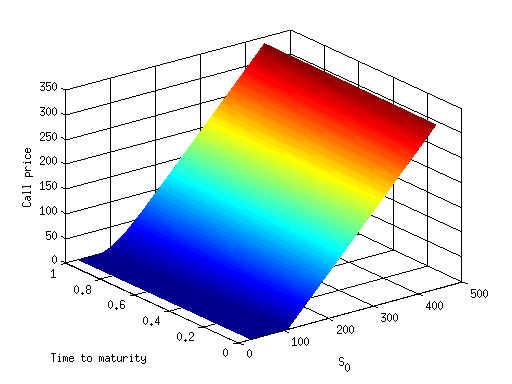
\includegraphics[scale=0.6]{3d.png}
\end{center}
\caption{A 3D plot of the results from FTCS with $\Delta X = \Delta \tau = 0.01$ for a call option with parameters: $r = 0.04, \sigma = 0.30, K = 110$ and $T = 1$.}
\label{fig:3d}
\end{figure}

In table \ref{tab:FTCS} the results are given using FTCS for three stock prices: one in the money ($S_0 = 120$, bottom value), one at the money ($S_0 = 110$, middle value) and one out of the money ($S_0 = 100$, top value) can be found. In table \ref{tab:stable} the stability parameter can be found obtained from equation \ref{eq:stable}.

\begin{table}[h]
\centering
\begin{tabular}{c|c|c|c}
  & $\Delta X$ = 0.1 & $\Delta X$ = 0.01 &$\Delta X$ = 0.001\\
  \hline
  &	9.6679	(0.546\%)	&										&										\\
  $\Delta \tau$ = 0.1 	&	15.1027	(0.171\%)	& $\times$					& $\times$ 					\\
  &	21.9035	(0.526\%)	&										&										\\
  \hline
  &	9.5171	(1.124\%)	&										&										\\
  $\Delta \tau$ = 0.01	&	14.9727	(1.021\%)	&	$\times$					&	$\times$					\\
  &	21.7213 (0.310\%)	&										&										\\
  \hline
  &	9.5044	(1.256\%)	&	9.6269	(0.016\%)	&										\\
  $\Delta \tau$ =0.001	&	14.9572	(1.133\%)	&	15.1287	(0.001\%)	&	$\times$					\\	
  &	21.7058 (0.381\%)	&	21.7963 (0.007\%)	&
\end{tabular}
\caption{This table shows the FTCS values: first the result for $S=100$ (out of the money), then $S=K=110$ (at the money) and lastly $S=120$ (in the money). Between brackets is the relative error to the analytical solution. When the value blows up, we denote it with a $\times$.}
\label{tab:FTCS}
\end{table}


\begin{table}[H]
  \centering
  \begin{tabular}{l || c | c | c}
    & $\Delta X$ = 0.1 & $\Delta X$ = 0.01 &$\Delta X$ = 0.001\\
    \hline
    $\Delta \tau$ = 0.1 & 0.6464 & $3.2 \; 10^4$ & $3.2 \; 10^8$ \\
    $\Delta \tau$ = 0.01 & 0.6717 & 289 & $3.2 \; 10^6$ \\
    $\Delta \tau$ = 0.001 & 0.9642 & 0.6401 & $3.2 \; 10^4$ \\
  \end{tabular}
  \caption{The stability parameter calculated by equation (\ref{eq:stable}) for different spatial and temporal scales.}
  \label{tab:stable}
\end{table}
The first thing that we notice about the table is that sometimes the solution blows up. In Table \ref{tab:stable} we have calculated the value of $\xi$ for the FTCS-scheme in equation (\ref{eq:stable}) for the given parameters (with $r = 0.04$ and $\sigma = 0.30$). We see indeed that the value of $\xi$ is below 1 when the values in Table \ref{tab:FTCS} are not blowing up. For values of $\xi$ much larger than 1 we see that we indeed get rubbish when we do the calculations to determine the option price. This shows that our derivation for the stability parameter is most likely correct. We did not check these results for the CN-scheme, as an estimate is not easily made because of the sine in the denominator, equation (\ref{eq:CN}). However, an analysis should show that the value of $\xi$ is below 1 for every reasonable possible combination of $\Delta \tau$ and $\Delta X$ since the scheme is supposed to be unconditionally stable.

Continuing with table \ref{tab:FTCS} we see that unless $\Delta \tau$ is smaller or equal to $\Delta X$ the solution is unstable. Making $\Delta \tau$ smaller does not always improve the solution. When $\Delta X$ becomes smaller (and $\Delta \tau < \Delta X$) the approximation improves a lot. An optimal mesh size is of course very subjective, but keeping in mind that deviations of less than a cent are relatively unimportant, choosing $\Delta X = 0.01$ and $\Delta \tau = 0.001$ seems an appropriate choice of parameters. It is also interesting to plot a spectrum of estimated option prices with FTCS, as well as the spectrum of absolute and relative errors, see figure \ref{fig:FTCS}. 

\begin{figure}[H]
  \centering
  \subfloat{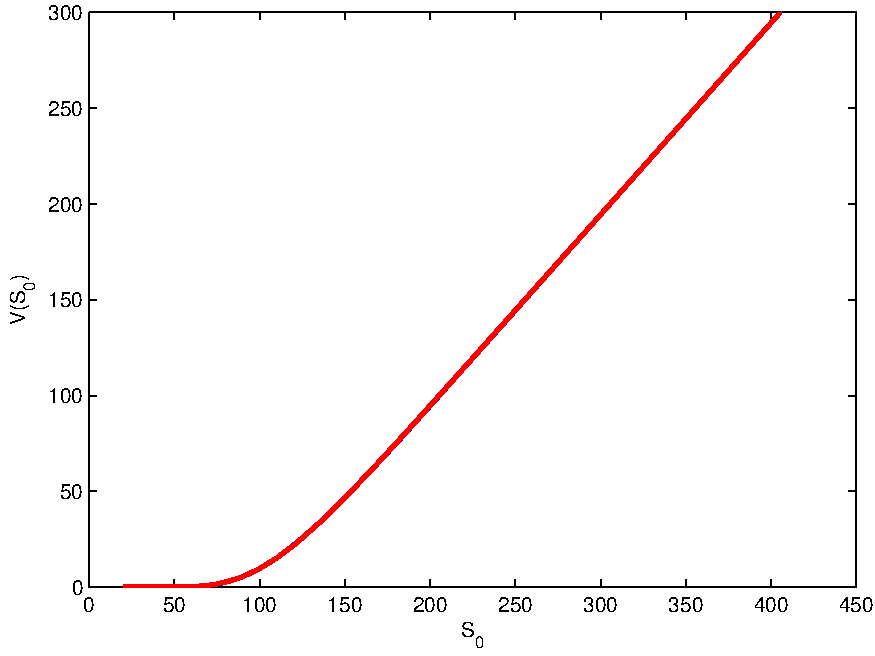
\includegraphics[width=0.39\textwidth]{PrijsFD01.pdf}}
  \subfloat{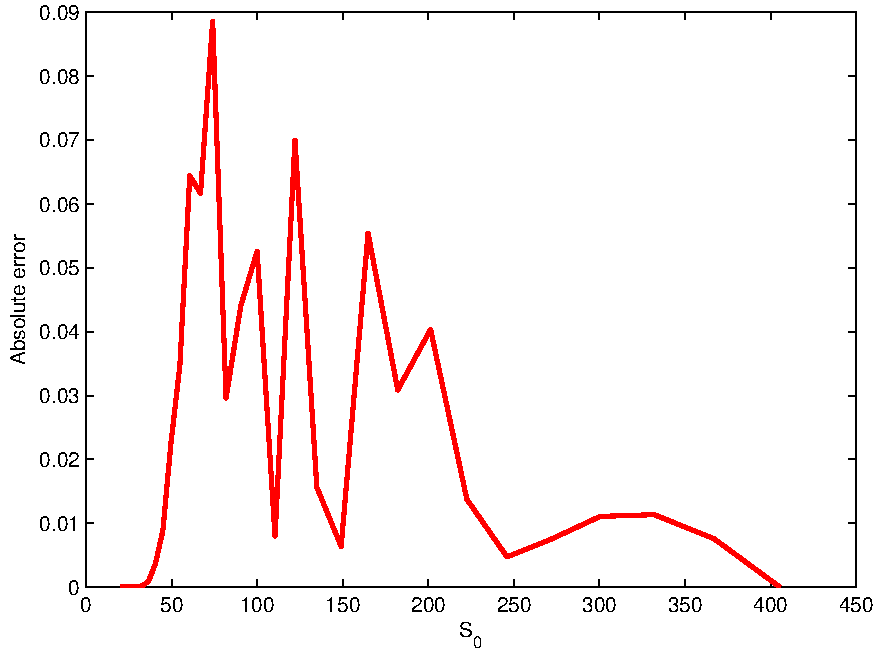
\includegraphics[width=0.39\textwidth]{AbsFoutFD01.pdf}} \\
  \subfloat{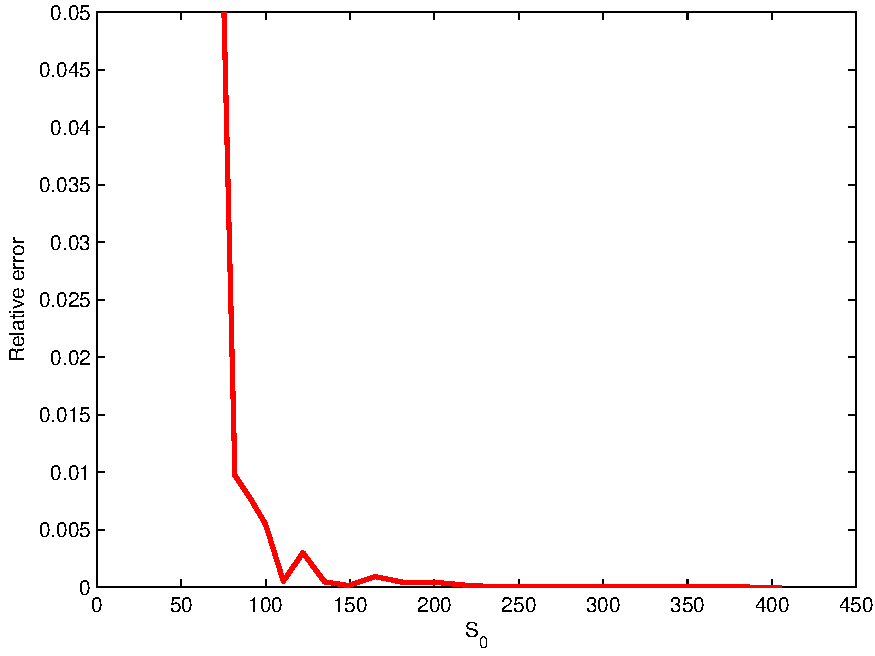
\includegraphics[width=0.39\textwidth]{RelFoutFD01.pdf}}
  \subfloat{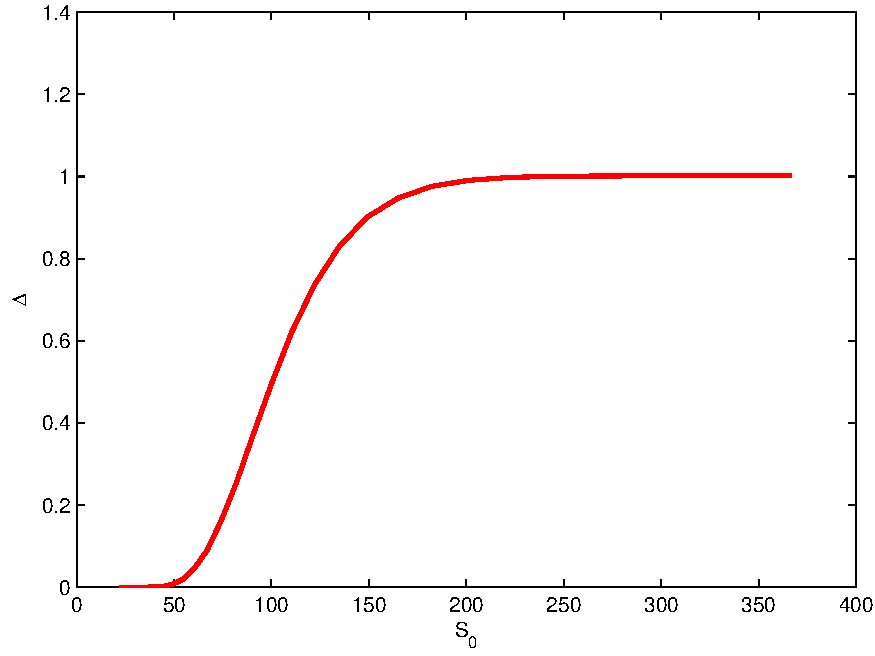
\includegraphics[width=0.39\textwidth]{DeltaFD01.pdf}}
  \caption{Obtained values with FTCS with $\Delta X=\Delta \tau=0.1$ for a call option with parameters: $r = 0.04, \sigma = 0.30, K = 110$ and $T = 1$. In the upper left corner are the call option values plotted (the blue line is the Black-Scholes solution), upper right the absolute error, lower left the relative error and lower right the estimated $\Delta$ from equation \ref{eq:Delta}.}
	\label{fig:FTCS}
\end{figure}

The call option price at time zero, $V(S_0)$, and $\Delta$ fits the exact solution well (the analytical call option price is plotted with a blue line, but is hard to see). The absolute error is low at the boundaries but fluctuates more in the other areas. This is why sometimes the estimation becomes worse when $\Delta \tau$ becomes smaller, despite the fact that the error bound decreases. One notices a relation between $\Delta$ and the absolute error. This relation is due to the fact that we are modelling the diffusion. We see that the absolute error is the biggest at the points with most diffusion, where $\Delta$ changes a lot, and lowest at the points with least diffusion where $\Delta$ is almost constant. The relative error peaks at low values, since for low values the difference between the estimation and analytical value is relatively bigger. We also see a peak at 110, which is caused by the diffusion which is centered around this point. Next we look at the results for the Crank Nicolson scheme, table \ref{tab:CNS}.

\begin{table}[h]
\centering
\begin{tabular}{c|c|c|c}
  & $\Delta X$ = 0.1 & $\Delta X$ = 0.01 &$\Delta X$ = 0.001\\
  \hline
  &	9.5060	(1.240\%)	&	9.6243	(0.012\%)	&	9.6238	(0.016\%)	\\
  $\Delta \tau$ = 0.1 	&	14.9598	(1.116\%)	& 14.8680	(1.722\%)	& 14.8048	(2.140\%)	\\
  &	21.7079	(0.372\%)	&	21.7852	(0.017\%)	&	21.7848	(0.018\%)	\\
  \hline
  &	9.5031	(1.240\%)	&	9.6255	(0.002\%)	&	9.6254	(0.000\%)	\\
  $\Delta \tau$ = 0.01	&	14.9554	(1.145\%)	&	15.1269	(0.011\%)	&	15.1023	(0.174\%)	\\
  &	21.7042	(0.389\%)	&	21.7886	(0.001\%)	&	21.7888	(0.000\%)	\\
  \hline
  &	9.5030	(1.271\%)	&	9.6255	(0.002\%)	&	9.6254	(0.000\%)	\\
  $\Delta \tau$ = 0.001	&	14.9555	(1.145\%)	&	15.1269	(0.011\%)	&	15.1286	(0.000\%)	\\	
  &	21.7041	(0.389\%)	&	21.7886	(0.001\%)	&	21.7888	(0.000\%)
\end{tabular}
\caption{This table shows the values for the CN-scheme: first the result for $S=100$ (out of the money), then $S=K=110$ (at the money) and lastly $S=120$ (in the money). Between brackets is the relative error compared to the analytical solution.}
\label{tab:CNS}
\end{table}

Contrary to the FTCS the solution is always stable. When $\Delta \tau$ becomes smaller the quality of the estimation improves when $\Delta \tau \leq \Delta X$. However when $\Delta \tau < \Delta X$, the estimation does not improve when $\Delta \tau$ becomes smaller. The same happens for $\Delta X$, when $\Delta X$ decreases the estimation improves when $\Delta X \leq \Delta \tau$ but does not improve much else wise. The most diffusion is at $S=K=110$. In the table we see this back when clearly $S=K=110$ has the biggest relative error (with $\Delta \tau, \Delta X \leq 0.01$). Thus an optimal choice for a mesh would be to have $\Delta t=\Delta X$ and choose them at least smaller then 0.01.

Next we plot the values and errors of the Crank Nicolson scheme for a range of values, figure \ref{fig:CN}. One sees that the call option value $V(S_0)$ and the Greek $\Delta$ match even better then FTCS. For the absolute error we just see a peak at 110, since there is the most diffusion. It is interesting to see that the absolute error is stable, i.e. it has no fluctuations as in the FTCS case. One notices again a relation between $\Delta$ and the absolute error. This relation is due to the fact that we are modelling the diffusion. We see that the absolute error is the biggest at the points with most diffusion, where $\Delta$ changes a lot, and lowest at the points with least diffusion where $\Delta$ is almost constant. The relative error peaks at low values and at 110, since for low values the difference between the estimation and analytical value is relatively bigger as with FTCS. The peak at 110 can be explained with the diffusion argument we saw before.

\begin{figure}[H]
  \centering
  \subfloat{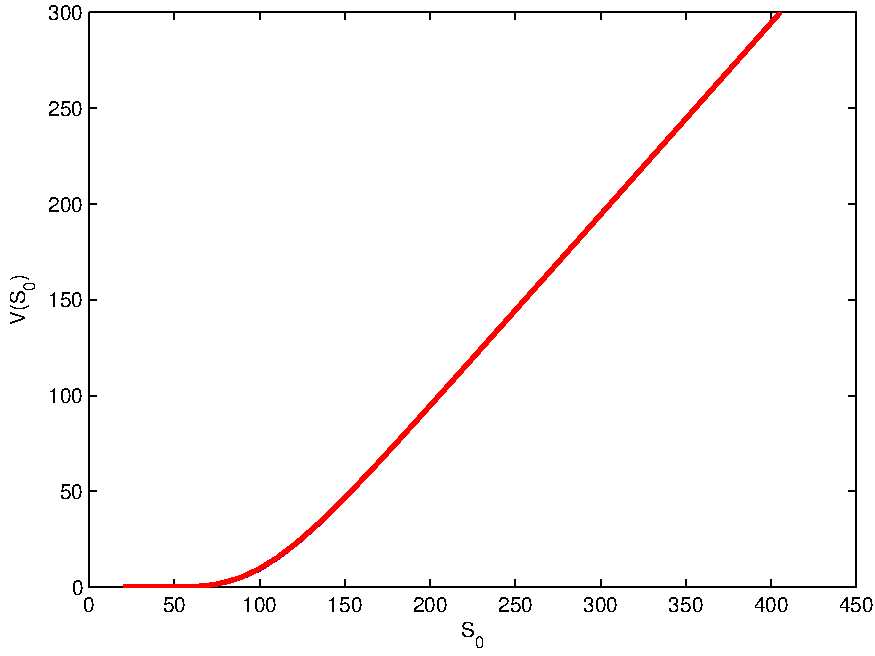
\includegraphics[width=0.39\textwidth]{PrijsCN01.pdf}}
  \subfloat{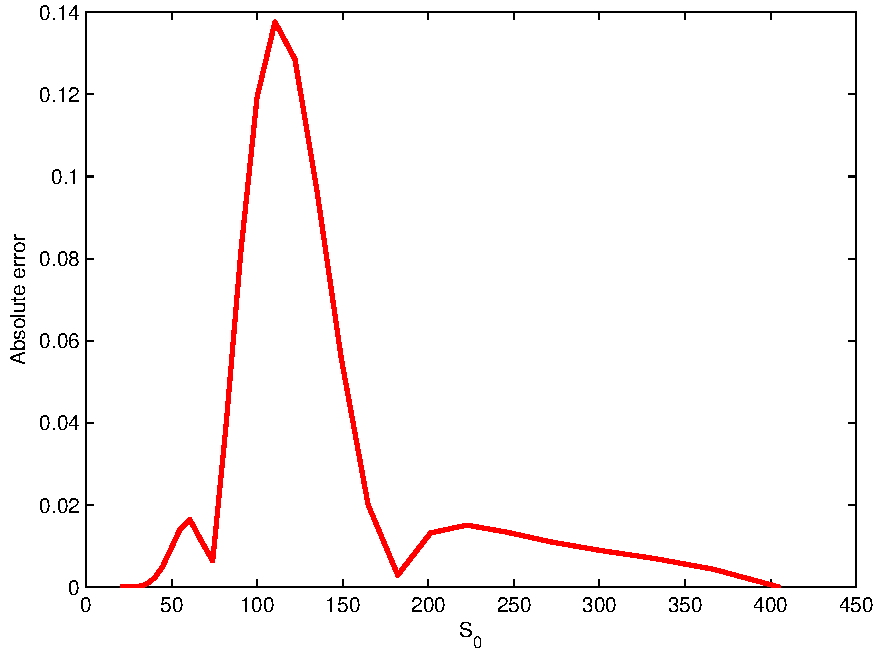
\includegraphics[width=0.39\textwidth]{AbsFoutCN01.pdf}} \\
  \subfloat{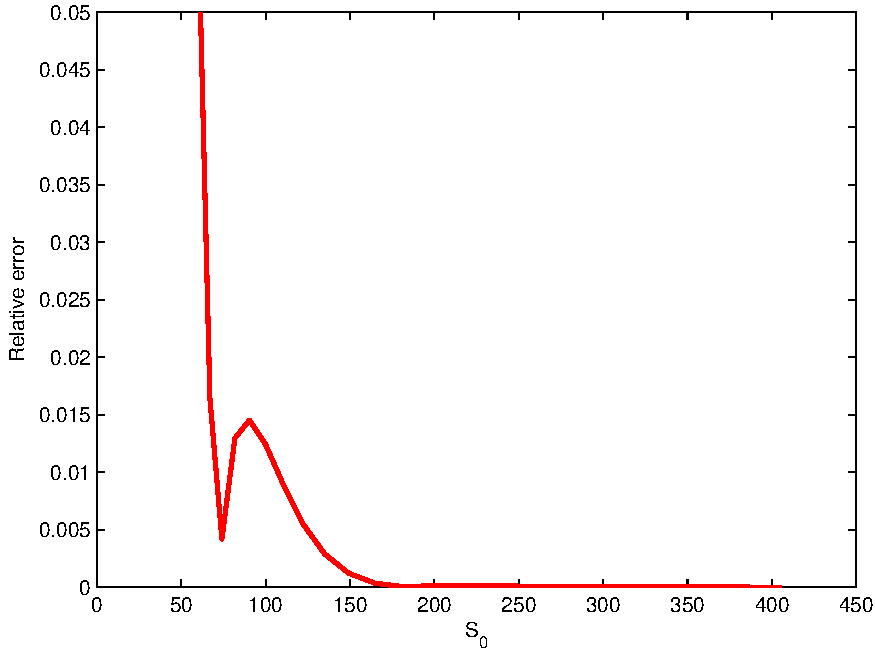
\includegraphics[width=0.39\textwidth]{RelFoutCN01.pdf}}
  \subfloat{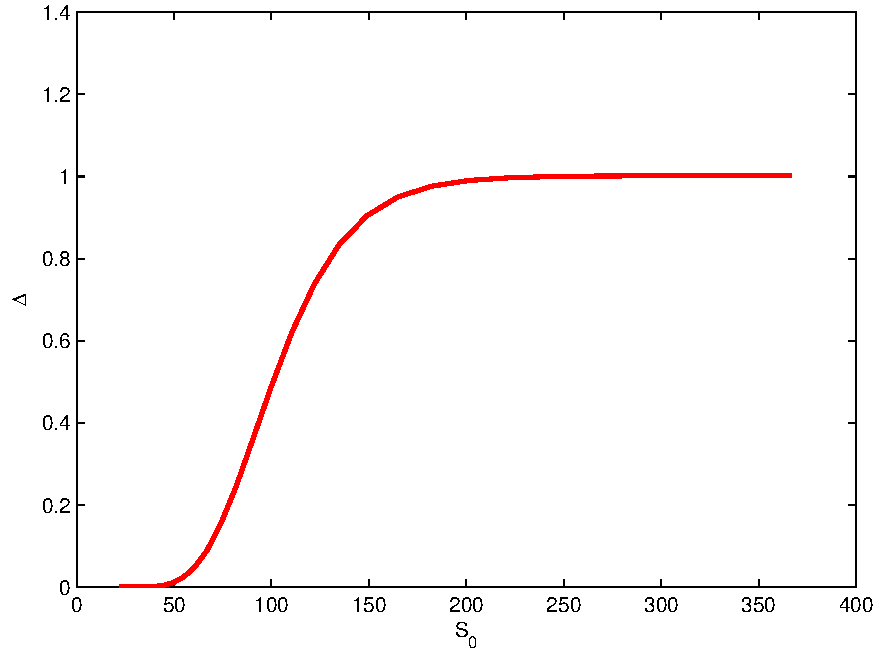
\includegraphics[width=0.39\textwidth]{DeltaCN01.pdf}}
  \caption{Computed values with CNS with $\Delta X=\Delta \tau=0.01$ for a call option with parameters: $r = 0.04, \sigma = 0.30, K = 110$ and $T = 1$. In the upper left corner are the call option values plotted, upper right the absolute error, lower left the relative error and lower right the values for $\Delta$.}
  \label{fig:CN}
\end{figure}

Lastly we look at a digital European style option which has a payoff of 1 if $S_T>K$ by simply changing the payoff function in the algorithm for FTCS. Figure \ref{fig:3dd} clearly shows the diffusion around $S_0=K$, where the payoff is a Heaviside function at $\tau = 0$ which more and more when $\tau$ increases.

\begin{figure}[h]
\begin{center}
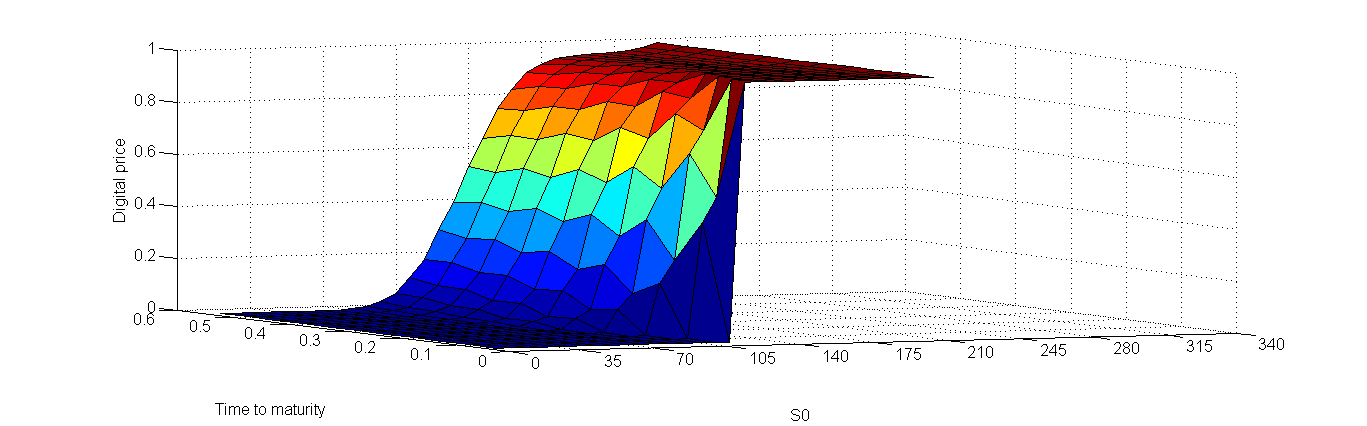
\includegraphics[scale=0.40]{3DD.png}
\end{center}
\caption{A 3D plot of the results from FTCS with $\Delta X = \Delta \tau = 0.01$ for a digital option with parameters: $r = 0.04, \sigma = 0.30, K = 110$ and $T = 1$.}
\label{fig:3dd}
\end{figure}

\section{Conclusion}
We investigated two finite difference schemes, the FTCS and the CNS, to price an European call option. We found that the FTCS scheme is conditionally stable and is outperformed by the CNS scheme, which is unconditionally stable, both methods converge well in the region in which they are stable. An advantage of a finite difference scheme is that it can handle exotic options and converge criteria are relatively easy to obtain. The schemes can also be used to derive the Greeks, of which we have seen $\Delta$ as an example. Lastly we looked at the behavior for a digital option and found a clear diffusion process for options at the money.

\begin{thebibliography}{10}
\bibitem{Isaacson}
  E. Isaacson, H.B. Keller, \emph{Analysis of numerical methods}, John Wiley and Sons, London \& New York, 1966 
\end{thebibliography}

\end{document}
